\documentclass[fr]{../../../eplnotes}

\usepackage{../../../eplunits}
\usepackage{bm}
\usepackage{interval}
\usepackage{multirow}
\usepackage{float}
\usepackage{xcolor}
\usepackage{enumitem}
\usepackage{tikzsymbols}
\usepackage{diagbox}
\usepackage{tablefootnote}

\usepackage{pifont}
\newcommand{\xmark}{\ding{55}}

%\usepackage{fontspec}
%\usepackage{algorithmicx}
%\usepackage{algpseudocode}
%\setmainfont{Hoefler Text}
%\newcommand*\Let[2]{\State #1 $\gets$ #2}
%\algrenewcommand\alglinenumber[1]{
%    {\sf\footnotesize\addfontfeatures{Colour=888888,Numbers=Monospaced}#1}}
%\algrenewcommand\algorithmicrequire{\textbf{Precondition:}}
%\algrenewcommand\algorithmicensure{\textbf{Postcondition:}}

\usepackage{pgfplots}
\pgfplotsset{width=7cm,compat=1.11}
\usepgfplotslibrary{fillbetween}
\pgfmathdeclarefunction{sqr}{0}{\pgfmathparse{0.2*x^2+1.2}}
\usetikzlibrary{arrows.meta}

\newcommand{\xb}{x_B}
\newcommand{\xn}{x_N}

\DeclareMathOperator{\epi}{epi}

\graphicspath{{img/}}

\hypertitle{Mod\`eles et m\'ethodes d'optimisation}{4}{INMA}{1702}
{Gilles Peiffer}
{François Glineur}

\paragraph{Remarque}
Chaque section reprend la matière d'un cours magistral.

\part{Partie linéaire}

\section{Introduction}

\subsection{Problème de Stigler}

	$x_i$ est la quantité du i\ieme{} aliment ($i = 1,\dots,77$).
	Le problème de Stigler s'écrit comme suit:
	\begin{equation*}
	\renewcommand{\arraystretch}{1.5}
	\begin{array}{c@{\quad} l c r@{\quad} l}
		\min\limits_{\bm{x}} & \sum\limits_{i = 1}^{77} c_i x_i & & & \\
		\textnormal{s.t.} & \sum\limits_{i = 1}^{77} A_{ij} x_i & \ge & b_j\,, & \forall j\,,\\
		& \multicolumn{1}{r}{x_i} & \ge & 0\,, & \forall i\,,
	\end{array}
	\end{equation*}
	où
	\begin{itemize}
		\item $c_i$ est le coût par unité de poids de $i$,
		\item $b_j$ est la quantité cible du nutriment $j$,
		\item $A_{ij}$ est la quantité du nutriment $j$
		dans l'aliment $i$ (par unité de poids).
		On a donc $A \in \R^{9 \times 77}$.
	\end{itemize}

	Notons que la première contrainte
	peut se réécrire en notation matricielle comme
	(par la suite,
	on omettra les notations spéciales pour les vecteurs et matrices):
	\[
	Ax \ge b\,.
	\]
	Dans cette équation,
	le signe ``$\ge$'' désigne
	l'\emph{element-wise greater than or equal to}
	(plus grand ou égal élément par élément).

	Notons également que ``s.t.'' est l'abbréviation de ``subject to''.

\subsection{Problème en deux dimensions}

	Montrons maintenant une façon graphique
	de résoudre un problème d'optimisation linéaire.
	Évidemment, cette méthode n'est à priori utile
	que pour les problèmes en deux dimensions.

	Soit le problème suivant:
	\begin{equation*}
	\begin{array}{c@{\quad} r c r c r@{\quad} l}
		\max\limits_{x} & x_1 & + & 2 x_2 & & &\\
		\textnormal{s.t.} & & & x_2 & \le & 6 &\\
		& x_1 & & & \le & 8 &\\
		& 3 x_1 & + & 4 x_2 & \le & 36 & \\
		& & & x_i & \ge & 0 & \forall i\,.
	\end{array}
	\end{equation*}

	Graphiquement, on obtient la figure suivante:

	\begin{center}
	\begin{tikzpicture}
		\draw[->,thick] (-1,0)--(9,0) node[right]{$x$};
		\draw[->,thick] (0,-1)--(0,7) node[above]{$y$};

		\coordinate (O) at (0,0);
		\coordinate (A) at (0,6);
		\coordinate (B) at (4,6);
		\coordinate (C) at (8,3);
		\coordinate (D) at (8,0);

		\draw[fill=red!5] (O) -- (A) -- (B) -- (C) -- (D) -- cycle;

		\draw[color=red,thick] (O) -- (A) node[midway, left] {$x_1 \ge 0$};
		\draw[color=red,thick] (A) -- (B) node[midway, above] {$x_2 \le 6$};
		\draw[color=red,thick] (B) -- (C) node[midway, above right] {$3x_1 + 4 x_2 \le 36$};
		\draw[color=red,thick] (C) -- (D) node[midway, right] {$x_1 \le 8$};
		\draw[color=red,thick] (O) -- (D) node[midway, below] {$x_2 \ge 0$};

		\draw [dashed, domain=1:5.5,samples=200, color=green!30] plot(\x,{10 - 0.5*\x});
		\draw [dashed, domain=1:5.5,samples=200, color=green!30] plot(\x,{9 - 0.5*\x});
		\draw [domain=1:5.5,samples=200, color=green] plot(\x,{8 - 0.5*\x});
		\draw [dashed, domain=1:5.5,samples=200, color=green!30] plot(\x,{7 - 0.5*\x});

		\node at (B) [circle,fill=green,inner sep=2.5pt] {};

	\end{tikzpicture}
	\end{center}

	Le point vert est appelé la solution optimale,
	alors que la surface rouge est appelée
	l'ensemble des solutions admissibles.

	Pour voir que le point vert est optimal,
	il suffit de proposer à la suite plusieurs valeurs optimales,
	jusqu'à se rendre compte qu'à chaque valeur optimale correspond
	une fonction objectif.
	On voit que le premier point de l'ensemble admissible atteint ainsi
	est bien le point vert.

\subsection{Problème de flots (ou de transport)}

	\begin{center}
	\begin{tikzpicture}
		\node [rectangle] (cij) at (-3,-3) {$c_{ij}$};
		\node [rectangle] (bitop) at (-3,0) {$b_{i}$};
		\node [rectangle] (bibottom) at (-3,-6) {$b_{i}$};

		\begin{scope}[every node/.style={circle,thick,draw,minimum size=1cm}]
			\node (P1) at (0,0) {$+10$};
			\node (P2) at (3,0) {$+5$};
			\node (P3) at (6,0) {$+10$};
			\node (C1) at (0,-6) {$-12$};
			\node (C2) at (3,-6) {$-5$};
			\node (C3) at (6,-6) {$-8$};

		\begin{scope}[>={Stealth[black]}, every node/.style={fill=white,circle}, every edge/.style={draw=red,very thick}]
			\path [->] (P1) edge[bend right=10] node {$5$} (C1);
			\path [->] (P1) edge node {$3$} (C2);
			\path [->] (P1) edge[bend left=16] node {$2$} (C3);
			\path [->] (P2) edge[bend right=18] node {$4$} (C1);
			\path [->] (P2) edge node {$7$} (C2);
			\path [->] (P3) edge[bend left=16] node {$\frac{1}{2}$} (C1);
			\path [->] (P3) edge node {$3$} (C2);
			\path [->] (P3) edge[bend left=20] node {$4$} (C2);
			\path [->] (P3) edge node {$1$} (C3);
		\end{scope}
		\end{scope}
	\end{tikzpicture}
	\end{center}

	Par convention, les arêtes non dessinées ont un coût infini.

	Le problème s'écrit sous forme mathématique comme suit:
	\begin{equation*}
	\begin{array}{c@{\quad} c c r c r@{\quad} l}
		\min\limits_{x} & \sum\limits_{{\displaystyle (i,j) \in \mathcal{E}}} c_{ij}x_{ij} &&&&& \\
		\textnormal{s.t.} & \sum\limits_{{\displaystyle j \suchthat (i,j) \in \mathcal{E}}} x_{ij} & - & \sum\limits_{{\displaystyle j \suchthat (j,i) \in \mathcal{E}}} x_{ji} & = & b_i\,, & \forall i\,,\\
		&&& x_{ij} & \ge & 0\,, & \forall i,j\,,
	\end{array}
	\end{equation*}
	où
	\begin{itemize}
		\item les $x_{ij}$ sont les quantités transportées de $i$ à $j$,
		\item les $c_{ij}$ sont les coûts unitaires de transport
		de $i$ à $j$,
		\item les $b_i$ sont les ``bilans'' des n\oe{}uds
		\item et $\mathcal{E}$ est l'ensemble des paires $(i,j)$.
	\end{itemize}

\subsection{Problème discret}

	Les problèmes discrets sont plus difficiles et plus coûteux
	au niveau du temps de calcul.
	Cela implique qu'on n'a plus le même problême que dans le cas continu.

\subsection{Problème d'affectation}
\label{sec:affectation}

	\begin{center}
	\begin{tikzpicture}
		\node [rectangle] (pers) at (-2.3,0) {personnes ($i$)};
		\node [rectangle] (taches) at (0,1.5) {tâches ($j$)};

		\draw[step=0.5cm,color=gray] (-1,-1) grid (1,1);
			\node at (-0.75,+0.75) {1};
			\node at (-0.25,+0.75) {0};
			\node at (+0.25,+0.75) {0};
			\node at (+0.75,+0.75) {0};
			\node at (-0.75,+0.25) {0};
			\node at (-0.25,+0.25) {0};
			\node at (+0.25,+0.25) {1};
			\node at (+0.75,+0.25) {0};
			\node at (-0.75,-0.25) {0};
			\node at (-0.25,-0.25) {1};
			\node at (+0.25,-0.25) {0};
			\node at (+0.75,-0.25) {0};
			\node at (-0.75,-0.75) {0};
			\node at (-0.25,-0.75) {0};
			\node at (+0.25,-0.75) {0};
			\node at (+0.75,-0.75) {1};
	\end{tikzpicture}
	\end{center}

	Le problème d'affectation revient à dire
	qu'on a un certain nombre de personnes
	qui peuvent chacune faire une parmi plusieurs tâches.
	La façon la plus efficace de représenter ce problème
	est à l'aide d'une matrice (appelée matrice d'affectation)
	qui dit si oui ou non une personne $i$
	fait la tâche $j\,$.
	Chaque tâche à un certain coût $p_i$ pour la personne $i\,$.
	Si la personne $i$ fait la tâche $j$, $x_{ij}$ vaut 1,
	sinon il vaut 0.
	Sous forme mathématique, on a
	\begin{equation*}
	\begin{array}{c@{\quad} r c l@{\quad} l}
		\min\limits_{x} & \sum\limits_{{\displaystyle (i,j) \in \mathcal{E}}} p_i x_{ij} &&&\\
		\textnormal{s.t.} & x_{ij} & \in & \{0, 1\}\,, & \forall i,j\,.
	\end{array}
	\end{equation*}
	où $\mathcal{E}$ est l'ensemble
	des paires (personne, tâche) possibles.
	Le problème d'affectation est donc à priori
	un problème de flots discret.


\section{Formes standard et géométrique}

\subsection{Problème d'affectation continu}

	Intéressons-nous maintenant
	à une formulation continue du problème d'affectation.

	La seule chose qui change
	par rapport au problème d'affectation discret (\sectionref{affectation})
	est la contrainte
	\[
	x_{ij} \in \{0, 1\} \quad \forall i,j\,.
	\]
	Comme on se trouve maintenant dans une situation continue,
	elle se transforme en
	\[
	x_{ij} \in \interval{0}{1} \quad \forall i,j\,.
	\]

\subsection{Forme géométrique}

	La forme géométrique est une certaine façon
	de représenter un problème d'optimisation linéaire.

	Par convention, un problème d'optimisation
	est un problème de minimisation.
	En effet, maximiser et minimiser sont équivalents,
	à condition de changer le signe:
	\[
	\max c^T x \iff -\min -c^T x\,.
	\]

	En ce qui concerne les contraintes,
	on essaie d'avoir un système de la forme
	\[
	\begin{tabular}{|ccccccccc|}
		\hline
		\multicolumn{9}{|c|}{$a_1$} \\
		\hline
		\multicolumn{9}{|c|}{$a_2$} \\
		\hline
		\multicolumn{9}{|c|}{\multirow{5}{*}{$A$}}
		\\
		&&&&&&&&\\
		&&&&&&&&\\
		&&&&&&&&\\
		&&&&&&&&\\
		\hline
		0 & 0 & 0 & 0 & \multicolumn{1}{|c|}{1} & 0 & 0 & 0 & 0 \\
		\hline
	\end{tabular}
	\cdot
	\begin{tabular}{|c|}
		\hline
		\multirow{9}{*}{$x$}
		\\
		\\
		\\
		\\
		\\
		\\
		\\
		\\
		\\
		\hline
	\end{tabular}
	\ge
	\begin{tabular}{|c|}
		\hline
		$b_1$ \\
		\hline
		$b_2$ \\
		\hline
		\multirow{5}{*}{$b$}
		\\
		\\
		\\
		\\
		\\
		\hline
		0 \\
		\hline
	\end{tabular}\,.
	\]
	On remarque que toutes les contraintes sont de la forme
	\[
	a_i^T x \ge b_i\,.
	\]
	Pour arriver à cela,
	il faut savoir transformer toute contrainte
	en une contrainte de cette forme.
	Plusieurs règles permettent d'arriver à ce résultat:
	\[
	a_i^T x \le b_i \iff -a_i^T x \ge -b_i\,,
	\]
	\[
	a_i^T x = b_i \iff a_i^T x \ge b_i \land -a_i^T x \ge -b_i\,.
	\]

	Notons que les contraintes de la forme
	\[
	a_i^T x \ne b_i
	\]
	ne sont pas admises car on ne peut pas les mettre sous la forme désirée.

	Par défaut, les $x_i$ sont dits ``libres'',
	c'est-à-dire qu'il n'y a pas de contrainte dessus à priori.

	Si on veut mettre une contrainte dessus, par exemple de la forme
	\[
	x_i \ge 0\,,
	\]
	il suffit de rajouter une ligne à la matrice $A$
	(la dernière ligne dans l'exemple).
	Évidemment, les règles de conversion sont ici aussi valables.

	Tout problème d'optimisation linéaire
	peut être mis sous forme géométrique.

\subsection{Forme standard}

	Un problème sous forme standard est également
	un problème de minimisation par défaut.
	Cependant, les contraintes deviennent maintenant des égalités.

	Il faut donc de nouveau une règle
	pour transformer les contraintes
	pour un problème sous forme géométrique
	en celles pour un problème standard:
	\[
	a_i^T x \ge b_i \iff a_i^T x - s_i = b_i \land s_i \ge 0\,.
	\]
	On rajoute donc des variables $s_i$ appelées
	``variables d'écart'' (\emph{slack variables}).

	Une autre différence entre les deux formes est
	que les variables ne sont plus libres
	lorsqu'on passe sous forme standard.

	Pour transformer une variable libre
	en une variable plus grande ou égale à zéro,
	il suffit de la scinder en deux:
	\[
	x_i = x_i^+ - x_i^- \quad \forall i\,,
	\]
	avec
	\[
	x_i^+, x_i^- \ge 0 \quad \forall i\,.
	\]

	Cependant, ceci n'est pas efficace
	car on double le nombre de variables.
	Heureusement, on peut se passer de cette augmentation de la complexité.
	Si on choisit une variable $x^-$ telle que
	\[
	x^- = x_1^- = x_2^- = \dots = x_n^- \ge 0\,,
	\]
	le prix à payer n'est que d'une seule variable.

	La forme géométrique et la forme standard sont donc équivalentes.

\subsection{Valeur absolue}

	Il peut arriver dans un problème d'optimisation
	que l'on soit confronté à une valeur absolue
	(notamment lorsqu'on fait de la \emph{régression linéaire}).

	Prenons par exemple la fonction objectif suivante:
	\[
	\min_x \abs{x_1} + x_2\,.
	\]
	Résoudre ce problème revient en fait à résoudre
	\[
	\left\{
	\renewcommand{\arraystretch}{1.5}
	\begin{array}{c@{\quad} r c r@{\qquad} l}
		\min\limits_x & x_1 & + & x_2 & \textnormal{si } x_1 \ge 0\\
		\min\limits_x & -x_1 & + & x_2 & \textnormal{sinon.}
	\end{array}
	\right.
	\]

	Cependant, dédoubler ne fonctionne que pour les petits problèmes,
	à peu de variables.

	Imaginons devoir résoudre le problème de minimisation suivant:
	\[
	\min_x \sum_{i=1}^{100} \abs{x_i - \alpha_i} \quad x,\alpha \in \R^{100}\,.
	\]
	Un problème équivalent est le problème
	\[
	\min_{x,t} \sum_{i=1}^{100} t_i\,,
	\]
	où l'on a posé que
	\[
	\abs{x_i - \alpha_i} \ge t_i\,.
	\]
	On transforme maintenant cette contrainte en une contrainte linéaire,
	de sorte à obtenir le problème suivant
	\[
	\renewcommand{\arraystretch}{1.5}
	\begin{array}{c@{\quad} l c r@{\qquad} l}
		\min\limits_{x,t} & {\displaystyle \sum_{i=1}^{100}} t_i &&&\\
		\textnormal{s.t.} & x_i - \alpha_i & \le & t_i & \forall i\\
		& x_i - \alpha_i & \ge & -t_i & \forall i\,.\\
	\end{array}
	\]
	On peut ensuite transformer ce problème
	pour le mettre sous forme géométrique ou standard,
	comme détaillé dans les sections précédentes.

	Cette méthode fonctionne car la valeur absolue est une fonction convexe.

\subsection{Normes}

	Il existe plusieurs normes possibles.
	Voici quelques exemples:

	\begin{itemize}
		\item la norme $\ell_1$ définie par
		\[
		\norm{x}_1 \coloneqq \sum_i \abs{x_i}\,;
		\]
		\item la norme $\ell_2$ définie par
		\[
		\norm{x}_2 \coloneqq \sqrt{\sum_i x_i^2}\,;
		\]
		\item la norme $\ell_p$ définie par
		\[
		\norm{x}_p \coloneqq \left(\sum_i \abs{x_i}^p\right)^{1/p}\,;
		\]
		\item la norme $\ell_\infty$ définie par
		\[
		\norm{x}_\infty \coloneqq \max_i \abs{x_i}\,.
		\]
	\end{itemize}


\section{Géométrie des polyèdres}

\subsection{Convexité d'un ensemble}

	\begin{mydef}[Convexité d'un ensemble]
		Un ensemble $\mathcal{S} \subseteq \Rn$ est dit convexe
		si et seulement si
		\[
		\renewcommand{\arraystretch}{1.5}
		\begin{tabular}{c@{\quad}l}
			\multirow{2}{*}{$\lambda x + (1 - \lambda)y \in \mathcal{S}\,,$}
			& $\forall \lambda \in \interval{0}{1}\,,$\\
			& $\forall x,y \in \mathcal{S}$\,.
		\end{tabular}
		\]

		\begin{figure}[H]
		\begin{subfigure}[t]{.45\linewidth}
		\centering
		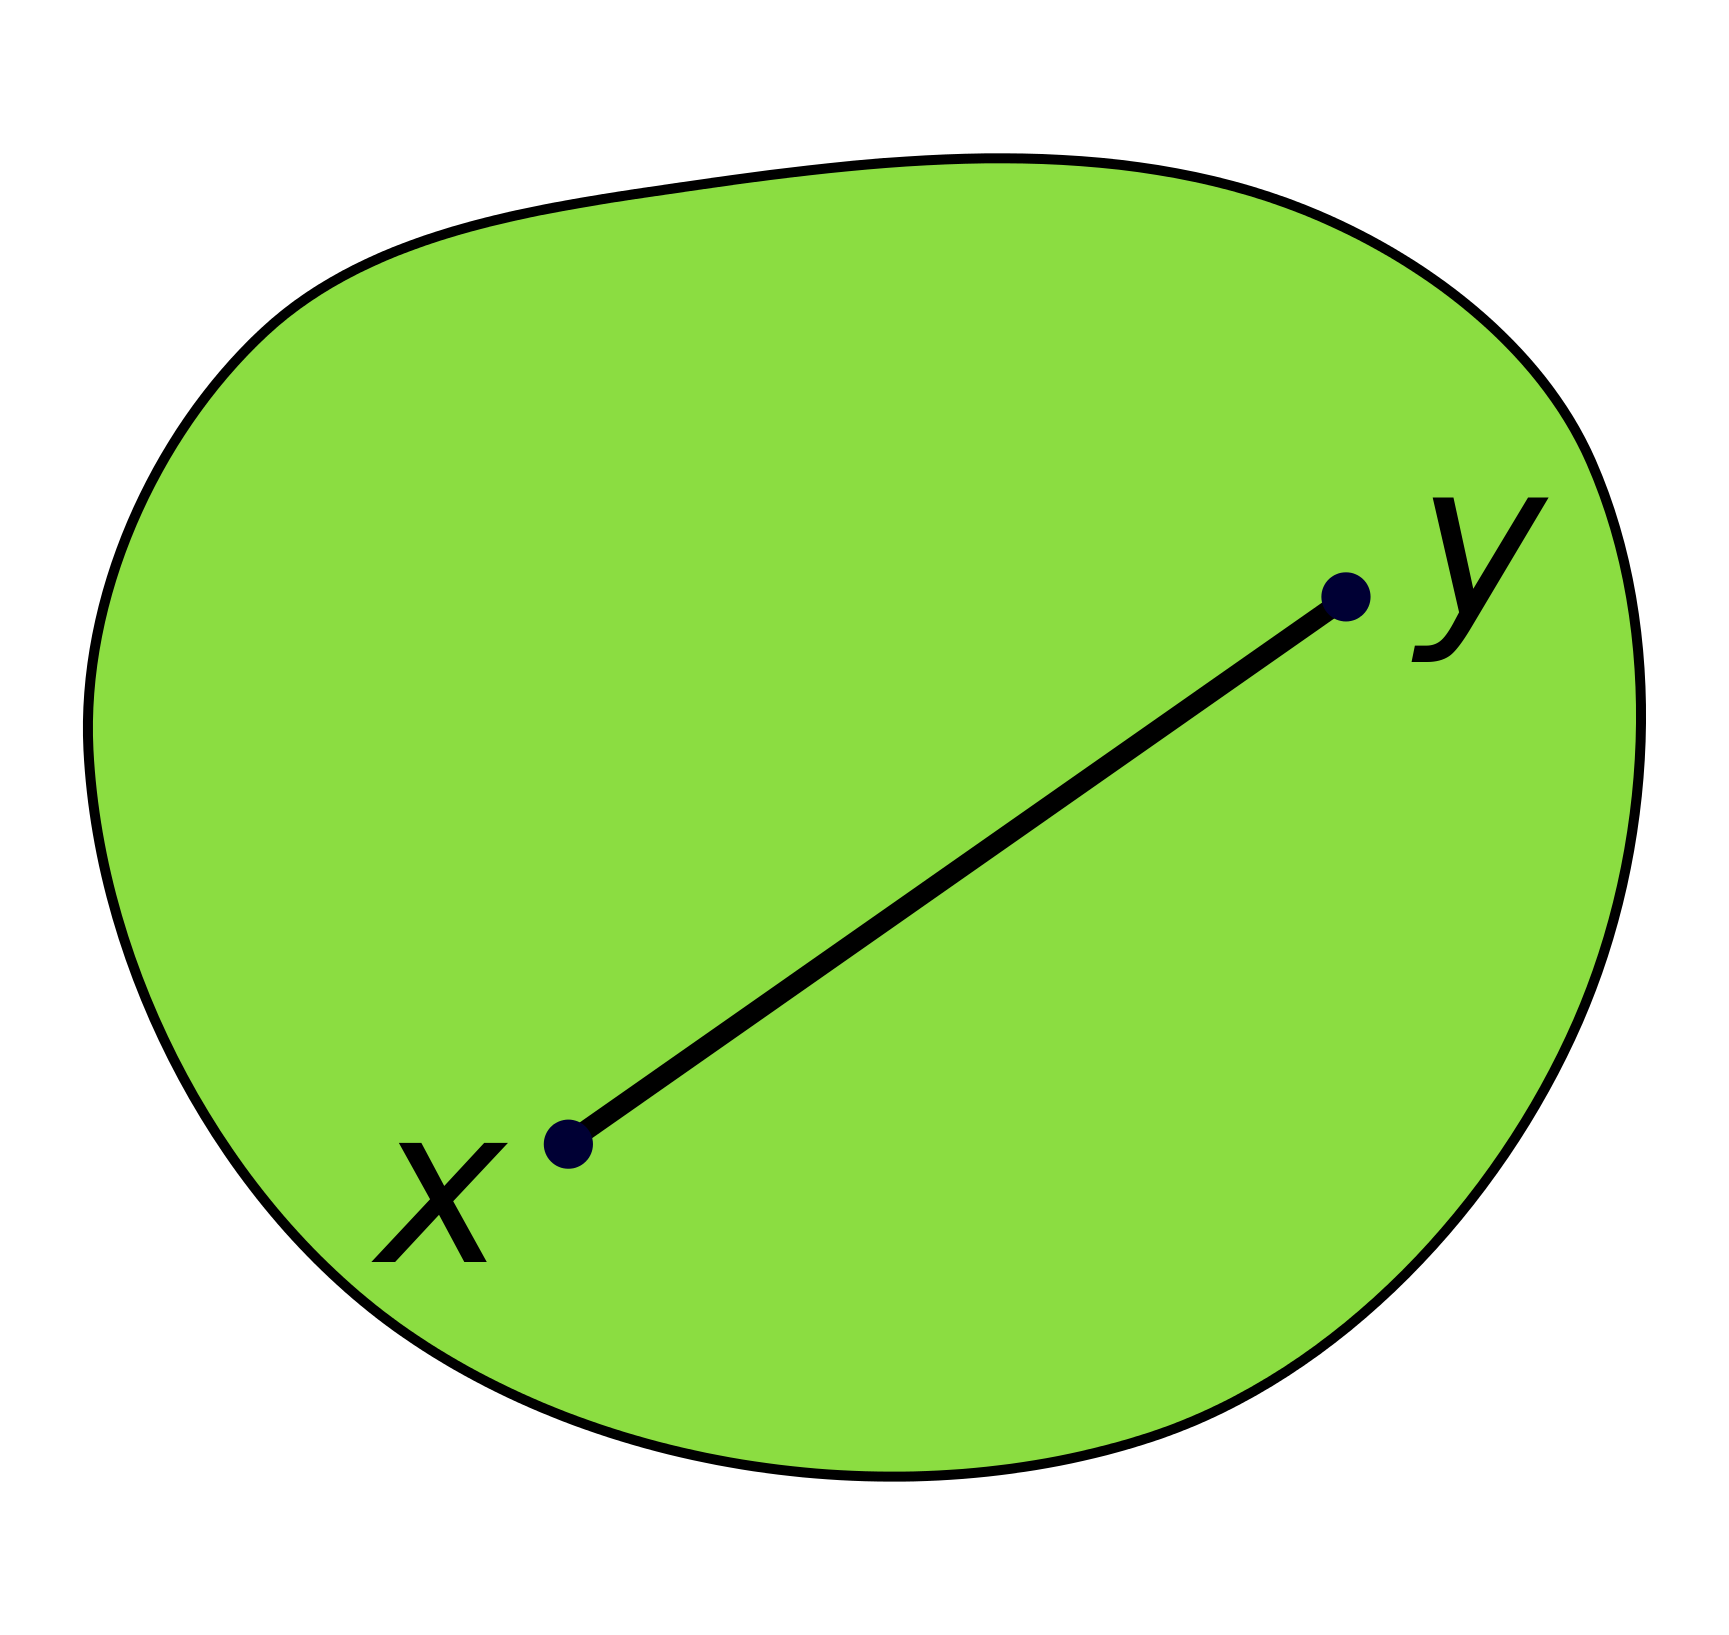
\includegraphics[width=\linewidth]{convex.png}
		\caption{Un ensemble convexe.
		Le segment de droite (noir) joignant les points $x$ et $y$
		est entièrement à l'intérieur de l'ensemble (vert).
		Comme ceci est vrai pour tous points $x$ et $y$ de l'ensemble,
		l'ensemble est convexe.}\label{fig:convex_set}
		\end{subfigure}%
		\hfill
		\begin{subfigure}[t]{.45\linewidth}
		\centering
		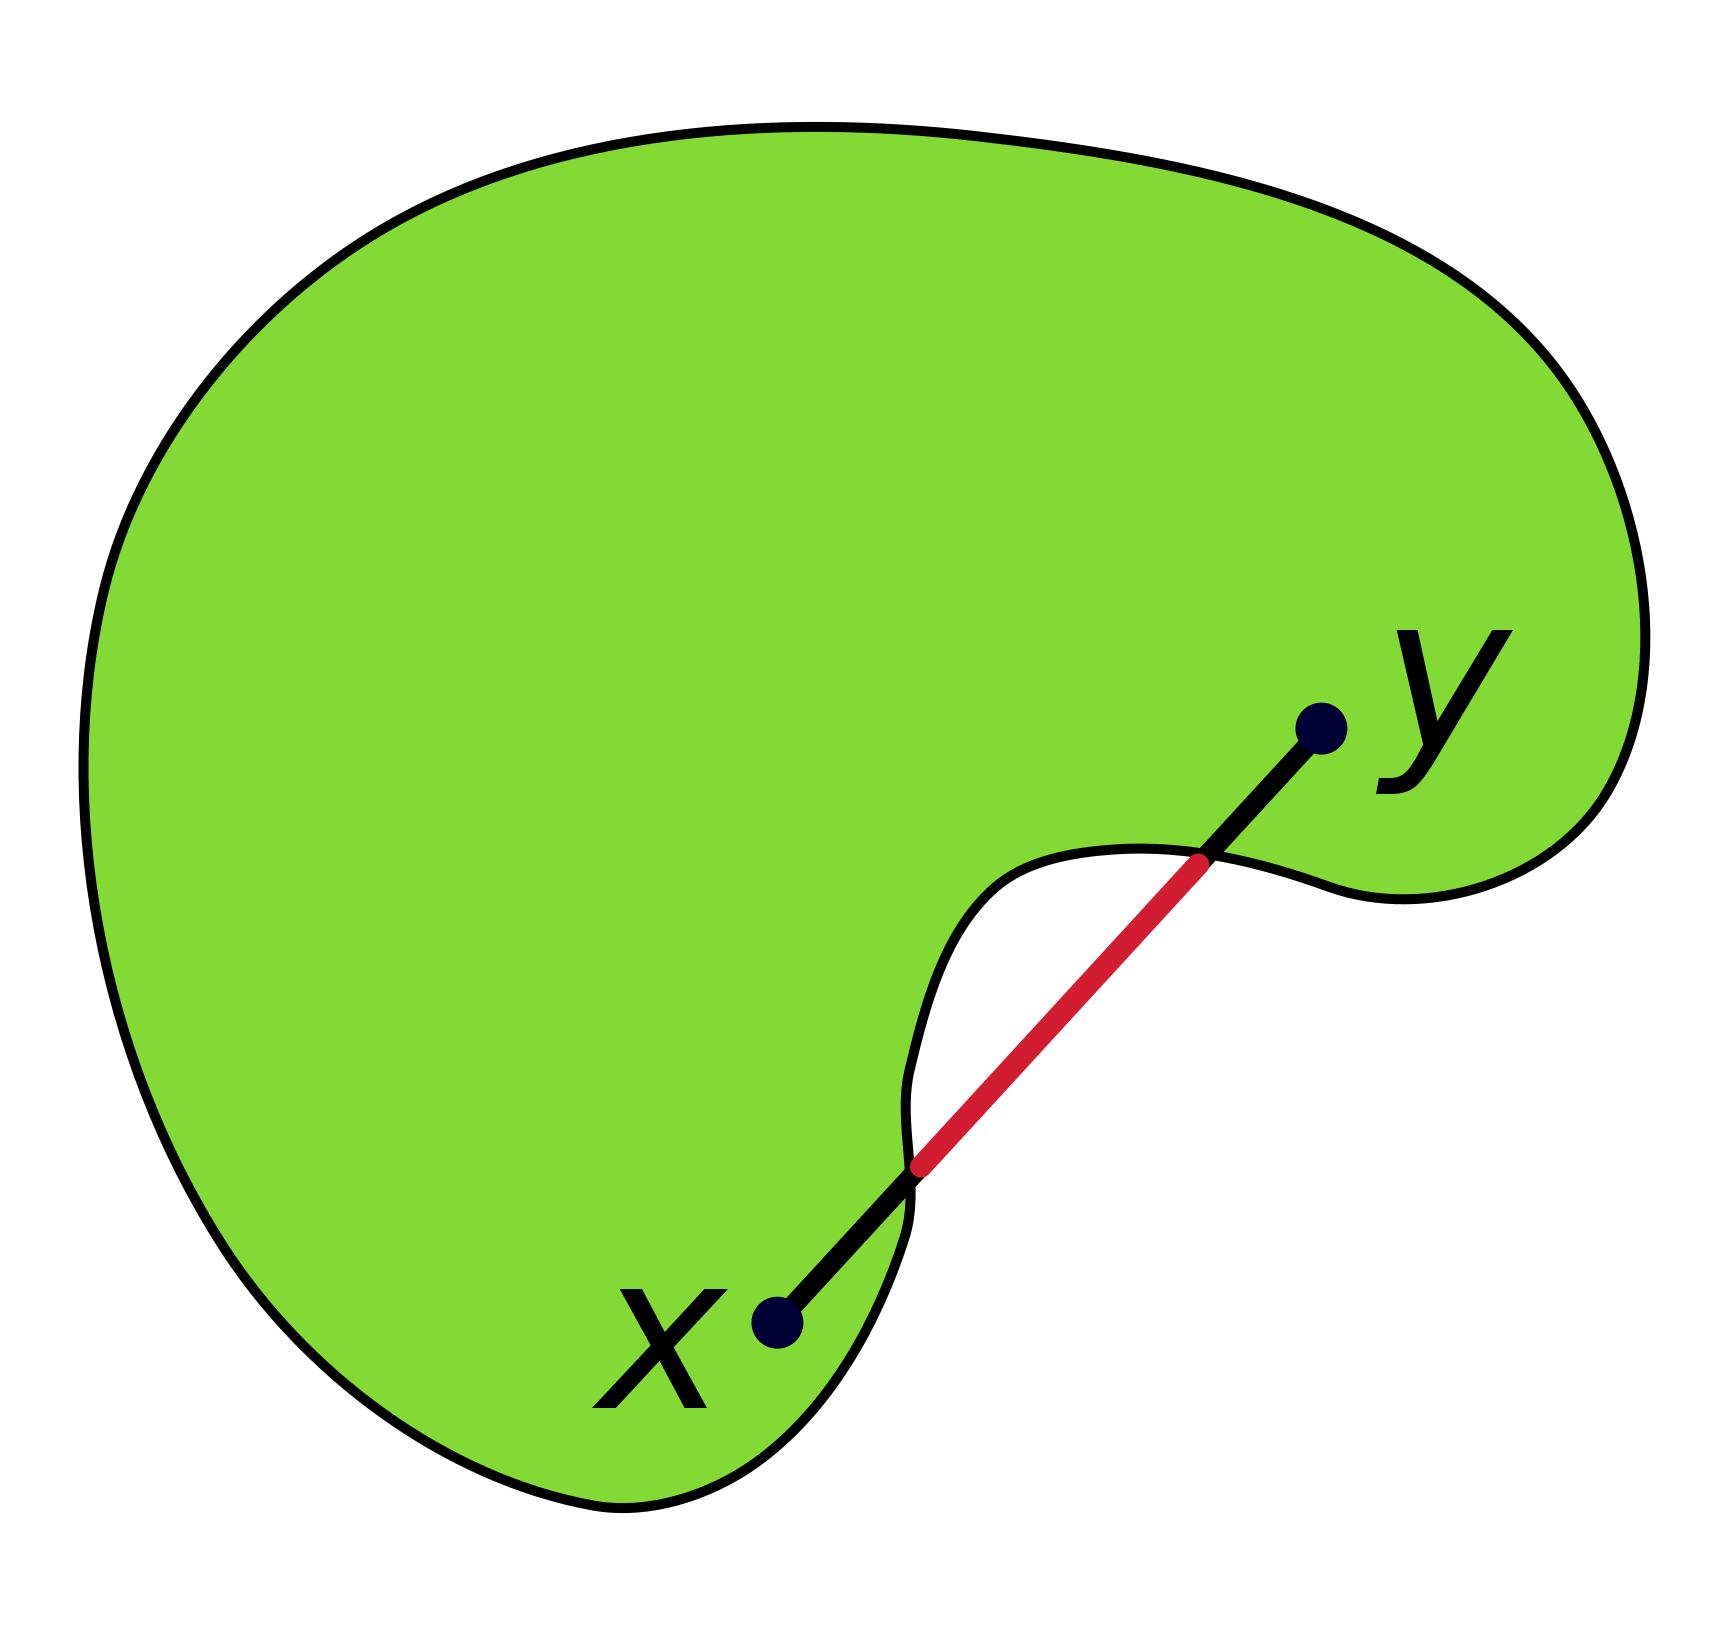
\includegraphics[width=\linewidth]{nonconvex.png}
		\caption{Un ensemble non convexe.
		Comme la partie rouge du segment de droite (noir et rouge)
		joignant les points $x$ et $y$
		est en dehors de l'ensemble (vert),
		l'ensemble est non convexe.}\label{fig:nonconvex_set}
		\end{subfigure}
		\caption{Exemples de convexité.}\label{fig:convexity}
		\end{figure}
	\end{mydef}

	\begin{mytheo}[Le demi-espace $\set{x \given a^T x \le b, a \ne 0}$ est convexe]\label{theo:demi-espace}\leavevmode
		\begin{proof}
			Si
			\[
			\left\{
			\begin{array}{c}
				a^T x \le b\,,\\
				a^T y \le b\,,
			\end{array}
			\right.
			\]
			alors a-t-on
			\[
			a^T \big(\lambda x + (1 - \lambda)y\big) \le b\,,
			\quad \forall \lambda \in \interval{0}{1}\,?
			\]

			Multiplions la première inéquation par $\lambda$,
			avec comme condition que $\lambda \ge 0$.
			Multiplions la seconde par $1-\lambda$,
			avec comme condition que $\lambda \le 1$.
			Additionnons maintenant les deux.
			On obtient alors l'inégalité suivante:
			\[
			a^T \big(\lambda x + (1 - \lambda)y\big) \le
			\lambda b + (1-\lambda) b\,.
			\]
			La partie à droite de l'inégalité se réduit facilement
			pour obtenir
			\[
			a^T \big(\lambda x + (1 - \lambda)y\big) \le b\,,
			\]
			ce qui prouve que le demi-espace est convexe.
		\end{proof}
	\end{mytheo}

	\begin{mytheo}[Convexité de l'intersection d'ensembles convexes]\label{theo:inter}\leavevmode
		Soient $\mathcal{S}_1$ et $\mathcal{S}_2$ convexes.
		Leur intersection $\mathcal{S}_1 \cap \mathcal{S}_2$
		est alors également convexe.

		\begin{proof}
			Soient $x,y \in \mathcal{S}_1 \cap \mathcal{S}_2$.

			\[
			\big(\lambda x + (1 - \lambda)y\big) \overset{?}{\subseteq} \mathcal{S}_1 \cap \mathcal{S}_2\,,
			\quad \forall \lambda \in \interval{0}{1}\,.
			\]

			Il suffit de montrer que

			\[
			\renewcommand{\arraystretch}{1.5}
			\begin{tabular}{c@{\quad}l}
				$\lambda x + (1 - \lambda)y \in \mathcal{S}_1\,,$ &
				$\lambda \in \interval{0}{1}$\\
				\multicolumn{2}{c}{et}\\
				$\forall \lambda x + (1 - \lambda)y \in \mathcal{S}_2\,,$ &
				$\forall \lambda \in \interval{0}{1}\,.$\\
			\end{tabular}
			\]
			On voit immédiatement
			que ces deux inclusions sont correctes,
			car les 2 ensembles sont convexes
			et que $x$ et $y$ appartiennent à leur intersection.
		\end{proof}
	\end{mytheo}

	\begin{mytheo}[Convexité de polyèdres]\leavevmode
		Tout polyèdre est convexe.
		\begin{proof}
			Comme un polyèdre est l'intersection
			d'un nombre fini de demi-espaces,
			en combinant le Théorème~\ref{theo:demi-espace}
			et le Théorème~\ref{theo:inter},
			on voit donc immédiatement
			que tout polyèdre est convexe.
		\end{proof}

		\begin{myrem}
			Notons que la réciproque n'est pas nécessairement vraie.
			En effet,
			prenons le contre-exemple de la boule unitaire:
			$\set{x \given \norm{x} \ge 1}\,.$
		\end{myrem}
	\end{mytheo}

\subsection{Convexité d'une fonction}

	\begin{mydef}[Convexité d'une fonction]\leavevmode
		Une fonction $f$ est dite convexe si et seulement si
		\[
		\set{(x,t) \given f(x) \le t}
		\]
		est convexe.
	\end{mydef}

	\begin{mydef}[Épigraphe d'une fonction]\leavevmode
		L'épigraphe d'une fonction $f \colon \Rn \to \R$
		est l'ensemble des points situés sur ou au-dessus
		du graphe de la fonction.

		Mathématiquement,
		\[
		\epi f = \set{(x,t) \given t \ge f(x)}\,.
		\]

		Graphiquement, on trouve ceci:

		\begin{center}
		\begin{tikzpicture}
		% this wasn't worth the effort it took...
		\begin{axis}[
			axis y line = middle,
			axis x line = middle,
			samples     = 200,
			domain      = -4.5:4.5,
			xtick       = \empty,
			ytick       = {3.7},
			yticklabels = {$t$},
			x label style={anchor=north},
			y label style={anchor=south},
			xlabel={$x \in \Rn$},
			ylabel={$f(x) \in \R$},
			xmin = -6, xmax = 6,
			ymin = -1, ymax = 6,
		]
			\addplot[name path=sqr, black, thick, mark=none, ] {sqr};
			\addplot[name path=line, gray, no markers, line width=0pt] {0.2*(4.5)^2+1.2};
			\addplot [
			color=green,
			fill=green,
			fill opacity=0.5
			]
			fill between[
			of = line and sqr,
			];
		\end{axis}
		\end{tikzpicture}
		\end{center}

		L'épigraphe est donc la partie verte du graphe.
	\end{mydef}

	Une fonction dont l'épigraphe est un polyèdre s'écrit
	\[
	f(x) = \max \left( a_i^T x - b_i \right)\,,
	\quad i \in \{1,2,\dots,n\}\,.
	\]

\subsection{Solutions}

	Prenons le système de contraintes
	\[
	\renewcommand{\arraystretch}{1.5}
	\left\{
	\begin{array}{rcl}
		x_1 & \ge & 0\,,\\
		x_2 & \ge & 0\,.
	\end{array}
	\right.
	\]
	Un point $(x_1,x_2)$ qui satisfait ces deux inéquations
	(comme par exemple $(1,1)$)
	est appelé une solution admissible de base.

	Prenons maintenant un système de contraintes différent:
	\[
	\renewcommand{\arraystretch}{1.5}
	\left\{
	\begin{array}{rcrcr}
		-x_1 & - & x_2  & \ge & -1\,,\\
		 x_1 & + & 2x_2 & \ge &  2\,.
	\end{array}
	\right.
	\]
	Le point $(0,1)$ satisfait ces deux inéquations
	de façon stricte.
	On dit que les contraintes sont ``actives'' ou ``serrées'' en $(0,1)$.
	Une solution admissible de base $x^* \in \Rn$ est dite dégénérée
	si le nombre de contraintes actives
	en $x^*$ est supérieur à $n$.

	\begin{center}
	\begin{tikzpicture}
		\begin{axis}[
			axis y line = middle,
			axis x line = middle,
			samples     = 200,
			domain      = -1:2.5,
			xtick       = {1,2},
			ytick       = {1},
			x label style={anchor=north},
			y label style={anchor=south},
			xlabel={$x_1$},
			ylabel={$x_2$},
			xmin = -2, xmax = 5.5,
			ymin = -1.5, ymax = 3,
		]
			\draw [orange, fill] (axis cs:0,1) circle [radius=2pt] node [above right] {dégénérée};
			\draw [red, fill] (axis cs:2,0) circle [radius=2pt] node [above right] {non admissible};

			\addplot[name path=c1, black, thick, mark=none, ] {1-x};
			\addplot[name path=c2, black, no markers, thick] {1-0.5*x};
			\addplot[name path=xaxis, gray, no markers, line width=0pt] {0};
			\addplot [
			color=green,
			fill=green,
			fill opacity=0.5
			]
			fill between[
			of = c1 and xaxis,
			soft clip={domain=0:1}
			];
		\end{axis}
	\end{tikzpicture}
	\end{center}

	Soit $\mathcal{P}$ un polyèdre.

	\begin{itemize}
		\item $\textnormal{$x$ est un point extrême de $\mathcal{P}$}
		\iff \nexists y,z \in \mathcal{P} \setminus \{x\} \suchthat x = \lambda y + (1 - \lambda) z\,,
		\quad \forall \lambda \in \interval{0}{1}\,.$
		\item $\textnormal{$x$ est un sommet de $\mathcal{P}$}
		\iff \exists c \suchthat c^T x > c^T y\,,
		\quad \forall y \in \mathcal{P} \setminus \{x\} \,.$
	\end{itemize}

\subsection{Variables de base et variables hors base}

	Prenons le système général suivant:
	\[
	Ax = b\,.
	\]
	On sait que

	\begin{itemize}
		\item $A$ est une matrice $m \times n$,
		\item $x$ est un vecteur colonne ($n \times 1$)
		\item et $b$ est un vecteur colonne également ($m \times 1$).
	\end{itemize}

	On a donc $m$ contraintes toujours serrées.
	Comme il faut serrer au moins autant de contraintes
	qu'il n'y a de variables,
	on serre également $n-m$ contraintes de type $x_i \ge 0$.

	Supposons sans perte de généralité que toutes les lignes de $A$
	sont linéairement indépendantes,
	c'est-à-dire que $m \le n$.

	On peut réarranger le vecteur $x$ de sorte à obtenir
	un vecteur scindé en deux selon que
	la variable $x_i$ soit égale à zéro ou pas.
	\[
	\begin{tabular}{l|c|}
		\cline{2-2}
		\multirow{3}{*}{$\xb$ ($m$ variables de base)} & \multirow{3}{*}{$\ge 0$}\\
		& \\
		& \\
		\cline{2-2}
		\multirow{5}{*}{$\xn$ ($n-m$ variables hors base)} & \multirow{5}{*}{$= 0$}\\
		& \\
		& \\
		& \\
		& \\
		\cline{2-2}
	\end{tabular}
	\]

	On doit alors scinder la matrice $A$ selon ces mêmes règles:
	\[
	A
	=
	\begin{bmatrix}
		B & N
	\end{bmatrix}\,.
	\]

	Après le choix de la base, $\xn = 0$.
	On trouve alors
	\[
	\renewcommand{\arraystretch}{1.5}
	\left\{
	\begin{array}{rcrcr}
		B \xb & + & N \xn & = & b\\
		      &   &   \xn & = & 0
	\end{array}
	\right.
	\iff
	\left\{
	\begin{array}{rcl}
		\xb & = & B^{-1} b\,,\\
		\xn & = & 0\,.
	\end{array}
	\right.
	\]

	$\xb = B^{-1} b \ge 0$ est une solution admissible de base
	si et seulement si
	$B$ a des colonnes linéairement indépendantes.


\section{Algorithme du simplexe}

\subsection{Algorithme}

Soit un problème d'optimisation linéaire sous la forme
\[
\renewcommand{\arraystretch}{1.5}
\begin{array}{c@{\quad}rcr@{\qquad}l}
	\max\limits_{x \in \Rn} & c^T x &     &      &                       \\
	\textnormal{s.t.}       &   A x & =   & b\,, & A \in \R^{m \times n} \\
	                        &     x & \ge & 0\,. &                       \\
\end{array}
\]

Reconstituons l'algorithme.

\begin{enumerate}
	\item \textbf{Recherche d'un sommet.}

	On a $m$ variables de base (dans $\xb$)
	et $n-m$ variables hors base (dans $\xn$).
	On a un sommet en $\begin{bmatrix} \xb & \xn \end{bmatrix}^T$,
	à condition que $\xn = 0$ et $\xb = B^{-1} b \ge 0$,
	avec $A = \begin{bmatrix} B & N \end{bmatrix}$.
	Cela veut donc dire que la matrice $B$ doit être inversible.
	\item \textbf{Recherche d'un sommet adjacent meilleur.}
	\begin{enumerate}
		\item \textbf{Regarder les sommets adjacents.}

		Un sommet adjacent est un sommet ayant
		une variable de différence dans la base $B$.
		\item Éventuellement, \textbf{choisir un sommet meilleur.}
	\end{enumerate}
	\item \textbf{Arrêt.}

	Si le programme s'arrête, on est à l'optimum.
\end{enumerate}

% TODO : Would've liked to include this but it seems to be a lot more complicated than it looks :(.
%
%\begin{algorithm}
%	\caption{Finding the vertex of the optimum solution to a linear programming problem}
%	\begin{algorithmic}[1]
%		\Require{$B$ is an invertible matrix}
%		\StateX
%		\Function{Simplex}{$A, b, c, x$}
%			\Let{$\xn$}{$0$}
%			\Let{$\xb$}{$B^{-1} b$} \Comment{$x$ is now a vertex}
%			\For{$x_{\textnormal{adj}}$ \gets every vertex adjacent to $x$}
%				\If{$c^T x_{\textnormal{adj}} > c^T x$}
%					\Let{$x$}{$x_{\textnormal{adj}}$}
%				\EndIf
%			\EndFor
%			\State \Return{$x$} \Comment{$x$ is now the vertex of the optimum solution}
%		\EndFunction
%	\end{algorithmic}
%\end{algorithm}

\subsection{Tableau du simplexe}

\begin{myexem}
	Considérons le problème suivant:
	\[
	\renewcommand{\arraystretch}{1.5}
	\begin{array}{c@{\quad}rcrcrcrcr@{\qquad}l}
		\min\limits_{x} &&& x_2 & - & 5 x_3 & + & 5 x_4 &&& \\
		\textnormal{s.t.} & x_1 & + & x_2 & - & 11 x_3 & + & 7 x_4 & = & 10\phantom{\,,} & \\
		&&& x_2 & - & 8 x_3 & + & 4 x_4 & = & 4\phantom{\,,} & \\
		&&&&&&& x_i & \ge & 0\,, & i \in \{1,2,3,4\}\,.
	\end{array}
	\]
	Construisons le tableau du simplexe pour ce problème.
	\[
	\renewcommand{\arraystretch}{1.5}
	\begin{array}{rrrr|r}
		x_1 & x_2 &  x_3 & \multicolumn{1}{r}{x_4} &    \\
		  0 &   1 &   -5 &                       5 &  z \\
		  \hline
		  1 &   1 &  -11 &                       7 & 10 \\
		  0 &   1 &   -8 &                      11 &  4
	\end{array}
	\]
\end{myexem}


\section{Dualité}

\subsection{Complexité de l'algorithme du simplexe}

Prenons le cas d'un problème à $n$ variables.
Une base de ce problème a donc $m$ indices
parmi ces $n$ variables.

Dans le pire des cas, le temps de résolution est
asymptotiquement exponentiel en $m$.

Cependant, pour la plupart des problèmes,
on trouve en pratique que la résolution est polynomiale
en $m$ et $n$.

Il existe aussi des algorithmes avec
une complexité polynomiale dans le pire des cas:
les méthodes de points intérieurs
(comme par exemple l'algorithme de Karmarkar).

\subsection{Dual}

Un problème d’optimisation linéaire
possède toujours un problème companion, un problème dual,
pour lequel le rôle des variables et des contraintes est inversé.
Le dual du dual est le problème initial
que l’on appelle problème primal.
Pour chaque variable dans le problème primal,
il y a une contrainte dans le dual
et pour chaque contrainte dans le problème primal,
il y a une variable dans le problème dual.

Ce problème dual permet notamment de trouver
la sensibilité par rapport au membre de droite.
C'est-à-dire que l'on peut estimer facilement
l'effet d'un changement de $b$ dans l'équation
$Ax = b$.

\subsection{Dualité faible/forte}

Soit $(P)$ un problème primal de minimisation.
Soit $(D)$ le problème dual de maximisation correspondant.

\begin{mytheo}[Théorème de la dualité faible]
	Si $x$ est admissible pour $(P)$ et a comme coût associé $p$
	et $y$ est admissible pour $(D)$ et a comme coût associé $d$,
	alors $p \ge d$.
	\begin{proof}
		Preuve par construction du dual.
	\end{proof}

	\begin{center}
		\begin{tikzpicture}
		\draw[->,thick] (0,0)--(0,6) node[above]{Objectif $\in \R$};
		\coordinate (A) at (0,0);
		\coordinate (B) at (0,6);

		\begin{scope}[>={Stealth[black]}, every node/.style={blue}]
		\node[label=0:$d_1$] (D1) at (0,0.5) {$\times$};
		\node[label=0:$d_2$] (D2) at (0,1.5) {$\times$};
		\node[label=0:$d^*$] (Dopt) at (0,2.5) {$\times$};
		\end{scope}

		\begin{scope}[>={Stealth[black]}, every node/.style={red}]
		\node[label=180:$p_1$] (P1) at (0,5.5) {$\times$};
		\node[label=180:$p_2$] (P2) at (0,4.5) {$\times$};
		\node[label=180:$p^*$] (Popt) at (0,3.5) {$\times$};

		\draw [decorate,decoration={brace,amplitude=10pt},xshift=-15pt,yshift=0pt]
		(-0.5,0.3) -- (-0.5,2.7) node [blue,midway,xshift=-1.8cm]
		{solutions duales};
		\draw [decorate,decoration={brace,amplitude=10pt,mirror, raise=15pt},yshift=0pt]
		(0.5,3.3) -- (0.5,5.7) node [red,midway,xshift=2.5cm]
		{solutions primales};
		\end{scope}
		\end{tikzpicture}
	\end{center}
\end{mytheo}

\begin{mycorr}
	Si $p^*$ est le coût optimal pour $(P)$
	et $d^*$ est le coût optimal pour $(D)$,
	alors $p^* \ge d^*$.
\end{mycorr}

\begin{mycorr}
	Si $x$ et $y$ sont tous les deux admissibles
	et vérifient $p = d$,
	alors ils sont tous les deux optimaux:
	\[
	(x,y,p,d) = (x^*,y^*,p^*,d^*)\,.
	\]
\end{mycorr}

\begin{mycorr}
	Si le primal est non borné,
	alors le dual est impossible.
	Si le dual est non borné,
	alors le primal est impossible.
\end{mycorr}

\begin{mytheo}[Théorème de la dualité forte]
	Si $(P)$ admet une solution optimale $x^*$,
	alors $(D)$ admet une solution optimale $y^*$
	telle que $p^* = d^*$.

	\begin{center}
		\begin{tikzpicture}
		\draw[->,thick] (0,0)--(0,6) node[above]{Objectif $\in \R$};
		\coordinate (A) at (0,0);
		\coordinate (B) at (0,6);

		\begin{scope}[>={Stealth[black]}, every node/.style={blue}]
		\node[label=0:$d_1$] (D1) at (0,1) {$\times$};
		\node[label=0:$d_2$] (D2) at (0,2) {$\times$};
		\end{scope}

		\begin{scope}[>={Stealth[black]}, every node/.style={red}]
		\node[label=180:$p_1$] (P1) at (0,5) {$\times$};
		\node[label=180:$p_2$] (P2) at (0,4) {$\times$};
		\end{scope}

		\begin{scope}[>={Stealth[black]}, every node/.style={magenta}]
		\node[label=180:$p^*$,label=0:$d^*$] (Popt) at (0,3) {$\times$};
		\end{scope}

		\draw [decorate,decoration={brace,amplitude=10pt},xshift=-15pt,yshift=0pt]
		(-0.5,0.8) -- (-0.5,3.2) node [blue,midway,xshift=-1.8cm]
		{solutions duales};

		\draw [decorate,decoration={brace,amplitude=10pt,mirror, raise=15pt},yshift=0pt]
		(0.5,2.8) -- (0.5,5.2) node [red,midway,xshift=2.5cm]
		{solutions primales};
		\end{tikzpicture}
	\end{center}
\end{mytheo}

\subsection{Classification}

\begin{table}[H]
	\centering
	\renewcommand{\arraystretch}{1.2}
	\begin{tabular}{|c|ccc|}
		\hline
		\diagbox[width=3.5cm]{$(P)$}{$(D)$} & Non borné & Solution optimale & Impossible\\
		\hline
		Non borné & \xmark & \xmark & \checkmark\\
		Solution optimale & \xmark & \checkmark & \xmark\\
		Impossible & \checkmark & \xmark & \checkmark\tablefootnote{Existe, mais numériquement instable.}\\
		\hline
	\end{tabular}
\end{table}

Pour une contrainte $a_i^T x \le b_i$
et la variable duale $y_i$,
on a une relation d'exclusion.
\begin{table}[H]
	\centering
	\begin{tabular}{c|cc}
		& $a_i^T x = b_i$ & $a_i^T x < b_i$\\
		\hline
		$y_i = 0$ & \checkmark & \checkmark\tablefootnote{Par exemple, imaginons avoir $\SI{24}{\hour}$ de disponible,
		mais une solution optimale avec $t \le \SI{24}{\hour}$.}\\
		$y_i > 0$ & \checkmark & \xmark
	\end{tabular}
\end{table}


\end{document}
